\subsection{Shannonova kapacita}


\df Domečkový součin grafů $G$ a $H$ je graf $G \boxtimes H$ takový, že:
\begin{align*}
	&V(G \boxtimes H) = \{ (u,v) \ |\  u\in V(G), v\in V(H) \} \\
	&E(G \boxtimes H) = \{ ((u_1,v_1),(u_2,v_2))\} \left\{\begin{matrix}
		&u_1 = u_2, v_1 \sim v_2 &\text{(sousedí)} \\
		&v_1 = v_2, u_1 \sim u_2 \\
		&v_1 \sim v_2, u_1 \sim u_2
		\end{matrix}\right.
\end{align*}

Motivací ke zkoumání Shannonovy kapacity grafu může být posílání zpráv.
Potřebujeme-li kód, který opraví jednu chybu, můžeme na $C_5$ najít pouze dvě
kódová slova ($\alpha(C_5) = 2$). Naproti tomu, $\alpha(C_5 \boxtimes C_5) = 5
> 2^2$. Posílání zpráv ve větších blocích tedy může být efektivnější.

\df Shannonova kapacida grafu:
$$\shn(G) = \sup_{i\ge 1}(\alpha(G^i))^{1/i}$$

\lm $\shn(G\boxtimes H) \ge \shn(G) \cdot \shn(H)$

\dk Vezměme si maximální nezávislou množinu v $G$ a maximální nezávislou
množinu v $H$. Z vlastností domečkového součinu plyne, že mezi vrcholy
$G\boxtimes H$ zkombinovanými z těchto množin nepovede žádná hrana a tudíž
budou tvořit nezávislou množinu velikosti alespoň $\alpha(G)\cdot\alpha(H)$.

\poz $\shn(G^i) \ge \shn(G)^i$

\dk Postupnou iterací lemmatu.

\df Ortonormální reprezentace grafu $G$ je funkce $\rho: V(G) \rightarrow \R^d$,
$\|\rho(v)\| = 1$. Pro každé $(u,v) \not\in E(G)$ platí $\rho(u)\bot\rho(v)$,
neboli $\sk{\rho(u), \rho(v)} = 0$.

\df Lovászova theta funkce:
$$\vartheta(G,\rho) = \max_{v\in V(G)} {1\over \sk{\rho(v),e_1}^2}$$

Vezmeme si reprezentaci grafu $C_5$ ta se skládá z pěti vektorů $v_1, \dots,
v_5$ a jednoho speciálního vektoru $e_1$, vůči kterému budeme ostatní
vztahovat. Protože se jedná o ortonormální reprezentaci, musí každé dva
nesousední vrcholy z $C_5$ svírat pravý úhel. Představíme si \uv{paraplíčko},
kde vektor $e_1$ tvoří držadlo a vektory $v_1, \dots, v_5$ jsou okolo něj a
tvoří dráty deštníku. Představme si dále, že deštník roztahujeme, dokud nebudou každé dva nesousední dráty svírat pravý úhel. Pak můžeme spočíst úhel mezi dráty a držadlem, který vyjde $\sk{\rho(v),e_1} = 5^{-{1\over 4}}$. Z toho:
$$
\vartheta(C_5,\rho) = \sqrt 5
$$

\begin{center}
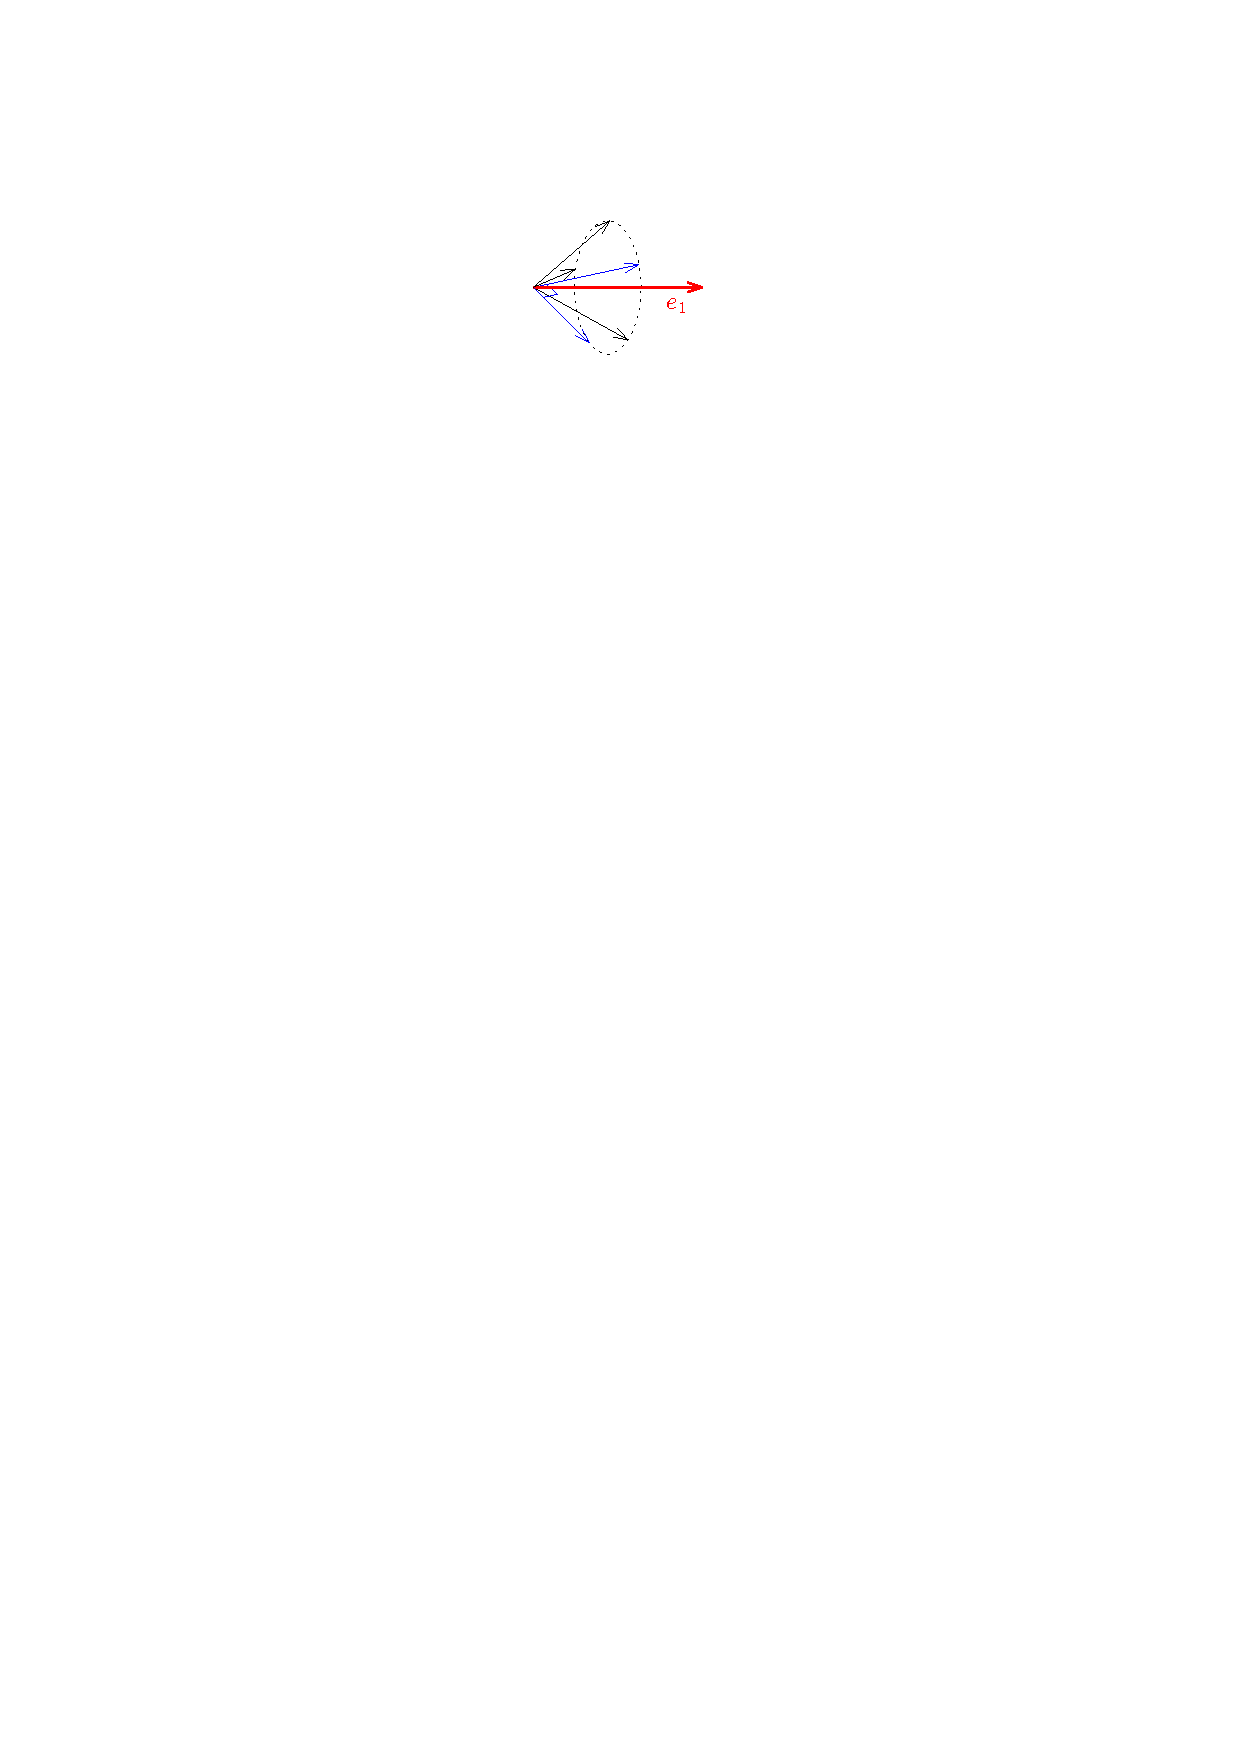
\includegraphics{lovaszovo_paraplicko.pdf}
\end{center}

\df $\vartheta(G) = \min\limits_{\rho\ \text{ONR}} \vartheta(G,\rho)$

Z toho plyne $\vartheta(C_5)\le \sqrt 5$. Kdybychom ještě znali vztah mezi
$\shn(G)$ a $\vartheta(G)$, měli bychom vyhráno. Tuto charakterizaci přináší
následující věta.

\vt $\shn(G) \le \vartheta(G)$

\dk K důkazu věty budeme potřebovat dvě pomocná lemmata.


\lm (O vztahu $\vartheta$ a $\alpha$) Nechť $H$ je graf a $\rho$ nějaká jeho ortonormální reprezentace. Pak $\alpha(H) \leq \vartheta(H, \rho)$.

\dk Nechť $A$ je nějaká nezávislá množina $H$. Zřejmě vektory $\rho(v)$ pro $v \in A$ tvoří ortonormální systém vektorů. Přáli bychom si odhadnout, jak velký bude skalární součin $\sk{\rho(v),e_1}^2$, z čehož nám vztah vyplyne.

Nechť $u$ je libovolný vektor a $b_i$ jsou vektory ortonormální báze. Chceme-li vyjádřit vektor $u$ proti bázi $b_i$, získáme $i$-tou souřadnici skalárním součinem $\sk{b_i,u}$ (můžeme si to představovat tak, že z vektorů $b_i$ složíme matici přechodu). Použijeme-li Pythagorovu větu, získáme:
\begin{align}
	||u||^2 = \sum_{i=1}^d \sk{b_i,u}^2
\end{align}
Pokud aplikujeme tento poznatek na vektory $\rho(v)$ rozšířené na bázi (což jistě lze), a vektor $e_1$, rovnost se změní na nerovnost (nezajímají nás přidané vektory) a s vědomím, že všechny vektory máme ortonormální, získáme:
\begin{align}
	1=||u||^2 \geq \sum_{v\in A}\sk{\rho(v),e_1}^2
\end{align}
Tedy existuje alespoň jeden vrchol $w$, že $\sk{\rho(w),e_1}^2 \leq 1/|A|$ a dosadíme-li do zlomku z definice $\vartheta$, získáme odhad $ \alpha(G) = |A| \leq\vartheta(H,\rho)$, což jsme chtěli dokázat. \qed



\lm (O součinu $\vartheta$) Nechť $H_1$ a $H_2$ jsou grafy, a $\rho_i$ jejich 
ortonormální reprezentace. Potom existuje ortonormální reprezentace $\rho$ 
silného součinu $H_1 \boxtimes H_2$, pro niž platí $\vartheta(H_1 \boxtimes H_2, 
\rho) = \vartheta(H_1, \rho_1) \cdot \vartheta(H_2,\rho_2)$.

\dk Zadefinujme si funkci $\rho$ pro vrcholy $v_i$ následovně:
\begin{align}
	\rho(v) = \rho_1(v_1) \otimes \rho_2(v_2)
\end{align}
Kde operace $\otimes$ je tenzorový součin vektorů, tedy pro $x \in \R^n$ a $y 
\in \R^m$ je výsledek vektor $z \in \R^{mn}$, který obsahuje všechny součiny 
$x_iy_i$. 

Zbývá pouze ověřit, že dělá správnou věc. Podívejme se tedy nejdříve na skalární 
součin:
\begin{align}
	\sk{x \otimes y , x' \otimes y'} = \sk{x,x'} \cdot \sk{y,y'}
\end{align}
Pokud levou a pravou stranu zvlášť rozepíšeme, je vidět, že roznásobením sum 
napravo získáme sumu nalevo a rovnost tedy platí:
\begin{align}
	\sum_{ij} (x_iy_j) \cdot (x_i' y_j') = \left( \sum_i x_ix_i'\right) \left(\sum_j 
	y_jy_j' \right)
\end{align}
Zde již jednoduchou úvahou zjistíme, že $\rho$ je stále ortonormální 
reprezentace: zjevně pro kolmé vektory jsou jejich tenzorové součiny opět kolmé, a všechny vektory si 
zachovají délku $1$. Nyní se stačí podívat, co se stane s $\vartheta$ funkcí, 
rozepišme si ji ted z definice:
\begin{align*}
	\vartheta(H_1 \boxtimes H_2, \rho) &= \max_{v\in V(H_1 \boxtimes H_2)} { 1 
	\over \sk{\rho(v) , e_1}^2} \\
	&= \max_{v\in V(H_1 \boxtimes H_2)} { 1 \over \sk{\rho_1(v_1)\otimes \rho_2(v_2) , e_{11} \otimes e_{12}}^2} \\
	&= \max_{v\in V(H_1 \boxtimes H_2)} { 1 \over \sk{\rho_1(v_1) , e_{11}}^2
		\cdot \sk{\rho_2(v_2) , e_{12}}^2} \\
	&= \max_{v_1\in V(H_1)} { 1 \over \sk{\rho_1(v_1) , e_{11}}^2} \cdot
	  \max_{v_2\in V(H_2)} { 1 \over \sk{\rho_2(v_2) , e_{12}}^2} 
	&= \vartheta(H_1,\rho_1) \cdot \vartheta(H_2, \rho_2)
\end{align*}
A lemma je dokázáno. \qed


\dk (Věty o vztahu $\Theta$ a $\vartheta$)  $$\alpha(G^i) \le \vartheta(G^i) \le \vartheta(G)^i$$
První nerovnost plyne z lemmatu o vztahu $\vartheta$ a $\alpha$. Druhá plyne z
opakovaného použití lemmatu o součinu $\vartheta$.
\qed


\lm (O dvojité kapacitě) $\shn(G + \overline{G}) \ge \sqrt{2|G|}$

\dk Ukážeme, že $\alpha ((G+\overline G)^2) \geq 2|G|$.
\begin{align*}
	V_{G+\overline G} = \{ v_1, ..., v_n, v_1', ..., v_n'\}
\end{align*}

Vezeme graf $(G+\overline G)^2$ a najdeme v něm nezávislou množinu $A$:
\begin{align*}
	A = \left\{\begin{matrix}
		(v_1, v_1'), (v_2, v_2'), \dots \\
		(v_1', v_1), (v_2', v_2), \dots
		\end{matrix}\right\}
\end{align*}

Velikost $A$ je zřejmě $2|G|$ a z definice Shannonovy kapacity dostaneme:
$$\shn(G + \overline{G}) \ge \sqrt{2|G|}$$
\qed


